
\title{The SVD and the Four Fundamental Subspaces}
\subtitle{\SubTitleName}
\institute[]{\Course}
\author{\Instructor}
\maketitle   


\frame{\frametitle{Topics and Objectives}
\Emph{Topics} \\
%\TopicStatement
\begin{itemize}

    \item the Singular Value Decomposition (SVD) of a matrix and the four fundamental subspaces

\end{itemize}

\vspace{0.5cm}

\Emph{Learning Objectives}\\

%\LearningObjectiveStatement

\begin{itemize}

    % \item compute the SVD for a rectangular matrix
    \item apply the SVD to construct bases for the four fundamental subspaces of a matrix
    %     \item construct a spectral decomposition of a matrix.
    % \end{itemize}
\end{itemize}

} 

\begin{frame}{The Four Fundamental Subspaces of a Matrix}



    % The idea behind this theorem is described in the diagram below. 
    \pause 
    
    \begin{center}
    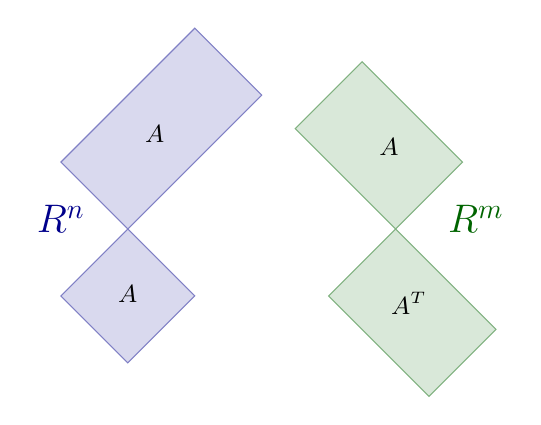
\begin{tikzpicture}[scale=.85]
        
        \onslide<2->{
        % boxes
        \filldraw[draw=DarkBlue!50,fill=DarkBlue!15] (0,0) -- (-1,1) -- (1,3) -- (2,2) -- cycle;
        \filldraw[draw=DarkBlue!50,fill=DarkBlue!15] (0,0) -- (1,-1) -- (0,-2) -- (-1,-1) -- cycle;      
        \draw (0.4, 1.7) node[below]{\small $\Row A$};
        \draw (0.0,-0.7) node[below]{\small $\Nul A$};        
        }
        
        \onslide<3->
        {
        \filldraw[draw=DarkGreen!50,fill=DarkGreen!15] (4,0) -- (2.5, 1.5) -- (3.5, 2.5) -- (5,1) -- cycle;
        \filldraw[draw=DarkGreen!50,fill=DarkGreen!15] (4,0) -- (5.5,-1.5) -- (4.5,-2.5) -- (3,-1) -- cycle;        
        \draw (3.9, 1.5) node[below]{\small $\Col A$};
        \draw (4.2, -0.8) node[below]{\small $\Nul A^T$};        
        }

        \onslide<4->{
        \draw (-1.0,0.5) node[below]{\Large $\color{DarkBlue} \mathbb R^n$};
        }

        \onslide<5->{
        \draw ( 5.2,0.5) node[below]{\Large $\color{DarkGreen} \mathbb R^m$};
        }
        
    \end{tikzpicture}\
    
    \vspace{12pt}
    \pause 
    The SVD of $A$ can be used construct bases for these subspaces. 
        
    \end{center}

\end{frame}

\begin{frame}{Recall: the SVD and the Four Fundamental Spaces}

Suppose $\vec v_i$ are orthonormal eigenvectors for $A^TA$, and $$\vec u _i = \frac{1}{\sigma_i}A\vec v_ i \ \text{ for } i \le r = \Rank A, \ \sigma_i = \lVert A \vec v_i \rVert.$$ Then we have the following bases for any $m\times n$ real matrix $A$. 
\begin{itemize}

    \item<2->  $ \vec v_1 ,\dotsc, \vec v_r$ is an orthonormal basis for $ \textup{Row} A$. 
    
    \item<2->  $ \vec v_{r+1} ,\dotsc, \vec v_n$ is an orthonormal basis for $ \Nul  A $. 
    
    
    \item<3->  $ \vec u_1 ,\dotsc, \vec u_r$ is an orthonormal basis for $ \textup{Col} A$.  
    
\end{itemize}

\vspace{12pt}

\onslide<4->{We can now also see that because $U$ is an orthogonal matrix, $ \vec u_{r+1} ,\dotsc, \vec u_m$ give an orthonormal basis for $ \Nul  A ^{T}$. }

\end{frame}


\begin{frame}\frametitle{Example}
    Given the SVD of $A$, determine $\text{rank}(A)$, and bases for $\Nul A$ and for $\Col A$.
    % \vspace{6pt} 
    \begin{align*}
        A = U \Sigma V^T = \spalignmat{0 1 0 0;0 0 1 0;0 0 0 -1;-1 0 0 0} \spalignmat{5 0 0 0 0;0 3 0 0 0;0 0 2 0 0;0 0 0 0 0} \spalignmat{0 0 \sqrt{0.8} 0 -\sqrt{0.2}; 1 0 0 0 0;0 1 0 0 0;0 0 0 1 0;0 0 \sqrt{0.8} 0 \sqrt{0.2}}
    \end{align*}

    \onslide<2->{\Emph{Solution} }
    \begin{itemize}
        \item<3-> there are exactly three non-zero singular values $\Rightarrow$ rank$A = 3$
        \item<4-> the last two columns of $V$ (or rows of $V^T$) are a basis for $\Nul A$
        \item<5-> first three columns of $U$ are a basis for $\Col A$
    \end{itemize}

\end{frame}


% \begin{frame} \frametitle{Example Solution}


% \end{frame}








\frame{\frametitle{Summary}

    \SummaryLine \vspace{4pt}
    \begin{itemize}\setlength{\itemsep}{8pt}

        \item applying the SVD to construct a bases for the four fundamental subspaces of a matrix

    \end{itemize}
    
    \vspace{6pt}
    \pause 
}



